% no answer key
% \documentclass[letterpaper]{exam}

% answer key
\documentclass[letterpaper, landscape]{exam}
\usepackage{2in1, lscape} 
\printanswers{}

\usepackage{units} 
\usepackage{xfrac} 
\usepackage[fleqn]{amsmath}
\usepackage{commath}
\usepackage{cancel}
\usepackage{float}
\usepackage{mdwlist}
\usepackage{booktabs}
\usepackage{cancel}
\usepackage{polynom}
\usepackage{caption}
\usepackage{fullpage}
\usepackage{comment}
\usepackage{enumerate}
\usepackage{graphicx}
\usepackage{mathtools} 

\newcommand{\degree}{\ensuremath{^\circ}} 
\everymath{\displaystyle}

\title{Algebra Notes \\ Section 3.5 and 3.6 }
\author{}

\date{\today}

\begin{document}

  \maketitle

  \section{Pythagorean Theorem} % (fold)

  \begin{figure}[H]
    \centering
    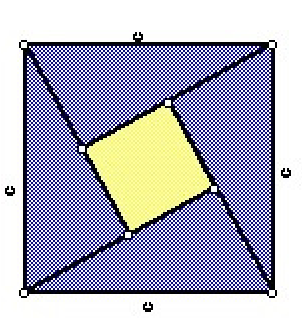
\includegraphics{proof.pdf}
    \caption{Pythagorean Theorem}
  \end{figure}
  
  The following figure was used by the Indian mathematician, Bhaskara (born 1114 CE) for another
  proof.  His proof was a little short on detail, as the entire proof was the figure and the phrase
  ``See!''.  

  The area of the big square is equal to the sum of the areas of the four triangles and the area
  of the small square.

  \begin{itemize*} 
    \item The area of each triangle is $\frac{1}{2} ab $.
    \item The area of the small square is $\del{ b - a }^2$.  
  \end{itemize*}

  \begin{align*} 
    c^2 & = 4 \del{ \frac{1}{2} ab } + \del{ b - a }^2 \\
        & = 2ab + b^2 - 2ab + a^2 \\
        & = a^2 + b^2 \\
  \end{align*}

  \section{Difference of Two Squares}

  examples:
  \begin{align*}
    x^2 - 1 \\
    x^2 - 4 \\
    9x^2 - 64 \\
    \del{x + 1}^2 - y^2 \\
    x^2y^2 - 9 \\
    1 - x^2y^2 \\
    7x - 28x^3 \\
  \end{align*}

  Mention sum of two squares can't be factored.

  \section{Sum/Difference of Two Cubes}

  formulas:
  \begin{align*}
    a^3 + b^3 &= (a + b) \del{a^2 - ab + b^2} \\
    a^3 - b^3 &= (a - b) \del{a^2 + ab + b^2} \\
  \end{align*}

  examples:
  \begin{align*}
    x^3 + 8 \\
    x^3 - 27 \\
    x^6 + y^6 \\
  \end{align*}
  
  \section{Factoring Trinomials} % (fold)

  Find numbers which add/subtract up to middle number and multiple to last number.

  Section 3.6: 1--5, 11--15, 21--25, 31--35, 41--45, 51--55, 70--79
  
\end{document}
